\section{Gazebo}
\label{section:gazebo}

Il toolbox di simulazione utilizzato, come precedentemente accennato, è Gazebo. Questo software permette di utilizzare un motore fisico interno del simulatore, denominato Open Dynamic Engine (ODE), \cite{ODE}. ODE è un motore fisico che permette di risolvere in tempo reale la dinamica degli oggetti posizionati all'interno del mondo di simulazione, determinando contemporaneamente lo stato di collisione, mantenendo la compatibilità con eventuali librerie aggiunte ed eseguite in contemporanea. Gazebo infatti mette a disposizione la sua Aplication Programming Interface (API), necessaria alla scrittura di codice sorgente per aggiungere funzionalità particolari come ad esempio la generazione dei dati da parte dei sensori e l'applicazione di forze aerodinamiche sul corpo del quadricottero, \cite{Gazebo}. 

Gazebo permette anche di utilizzare l'insieme di framework di Robot Operating System 2 (ROS2), della quale lo stesso Gazebo fa parte, includendo quindi una vastità di funzionalità e prodotti già implementati per applicazioni di robotica, \cite{ROSGAZEBO}.

All'interno progetto di sviluppo del firmware di PX4, \cite{PX4FIRMWARE}, è presente un esempio di simulazione utilizzando Gazebo, con relativi codici sorgenti di plugin utili nella cartella "Tools/sitl\_gazebo". Nella simulazione di default sono già presenti le funzionalità dei sensori, IMU e GPS, e l'interfaccia di comunicazione utilizzante il protocollo MavLink attraverso la rete locale del computer Host, Figura (\ref{fig:ig:INTERSIL}).
Per effettuare le simulazioni SIL all'interno del progetto è stato aggiunto il modello tridimensionale del drone, Figura (\ref{fig:DRONECAD}). Modificando i file di configurazione di gazebo sono stati assegnati i valori di massa e inerzia coerentemente come in tabella (\ref{tab:DRONE}).
E stato inoltre modificato il file del codice sorgente relativo al modulo software "gazebo\_motor\_model.cpp", come è possibile visionare in appendice, per implementare nella simulazione le leggi polinomiali trovate sperimentalmente riguardante le forze e i momenti sui rotori, Figura (\ref{fig:pwmTM}), in modo da avere un confronto più preciso con le simulazione effettuate in MIL.

\begin{figure}
	\centering
	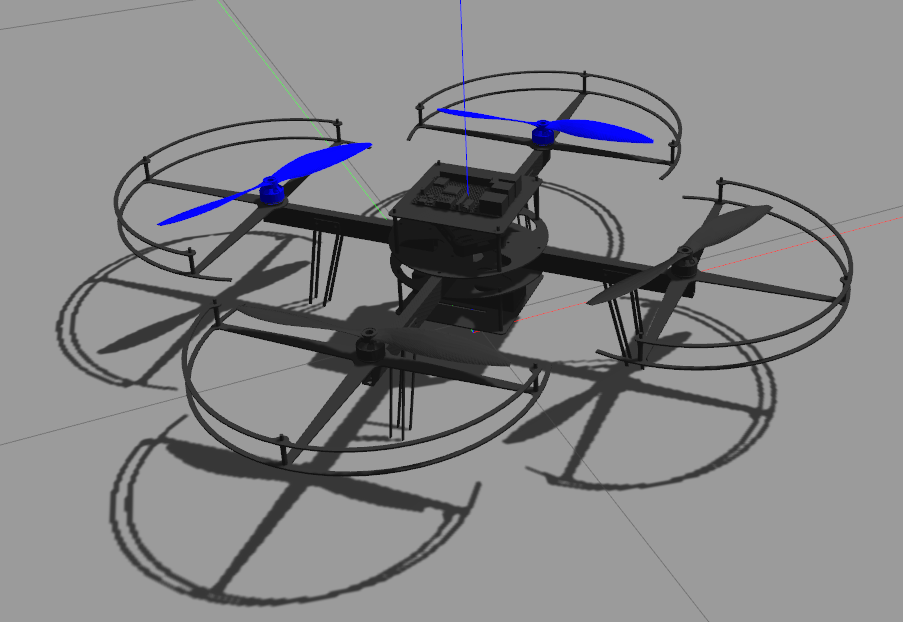
\includegraphics[width=0.4\textwidth]{DescrizioneAutopilota/Figure/DRONECAD}
	\caption{Drone utilizzato nella simulazione in Gazebo}
	\label{fig:DRONECAD}
\end{figure}

Il lancio della simulazione, avviene in contemporeanea al lancio del software di PX4 attraverso l'utilizzo di uno script., allegato in appendice. Questo script richiama il software con le corrette impostazioni ed avvia la simulazione collegando il simulatore al programma dell'autopilota.
